\section{Statische Grundglieder (ohne Gedächtnis)}

Der Ausgang des Systems ist \textbf{nur} vom aktuellen Eingang abhängig 
$$ y(t) = f( u(t) ) $$
\textbf{Hinweis:} $u(t)$ entspricht meist $A \cdot \varepsilon(t)$ (skalierter Einheitssprung)


\subsection{P-Glied (Proportional)}{26}

$$ \boxed{ y(t) = K \cdot u(t) } $$

\begin{minipage}{0.23\columnwidth}
    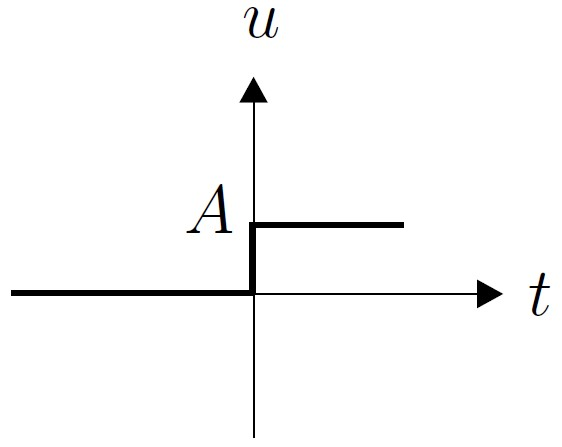
\includegraphics[width=0.8\columnwidth]{images/eingangssignal_schrittantwort.jpg} 
\end{minipage}
\hfill
    \begin{minipage}{0.23\columnwidth}
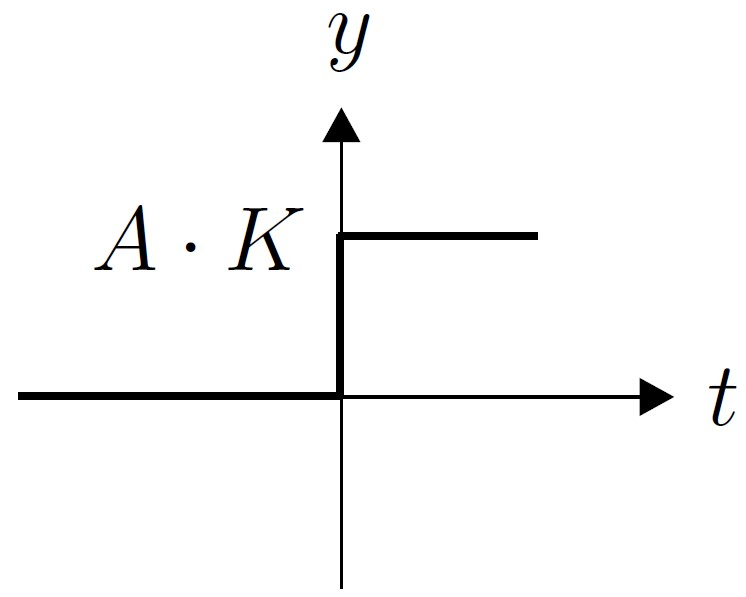
\includegraphics[width=0.8\columnwidth]{images/schrittantwort_p-glied.jpg} 
\end{minipage}
\hfill
\begin{minipage}{0.23\columnwidth}
    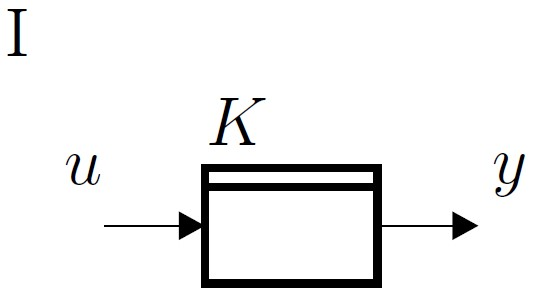
\includegraphics[width=0.8\columnwidth]{images/symbol_p-glied_1.jpg}
\end{minipage}
\hfill
\begin{minipage}{0.23\columnwidth}
    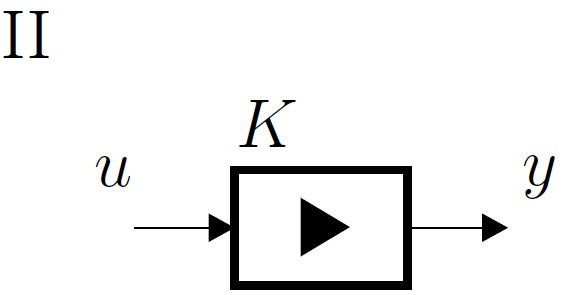
\includegraphics[width=0.8\columnwidth]{images/symbol_p-glied_2.jpg}
\end{minipage}


\subsection{Kennlinie / Pseudostatische Kennlinie}

\begin{minipage}[t]{0.25\columnwidth}
    \begin{center}
        \subsubsection{Kennlinie}

        \vspace{-0.4cm}
        $$ \boxed{ y(t) = f(u) } $$
        
        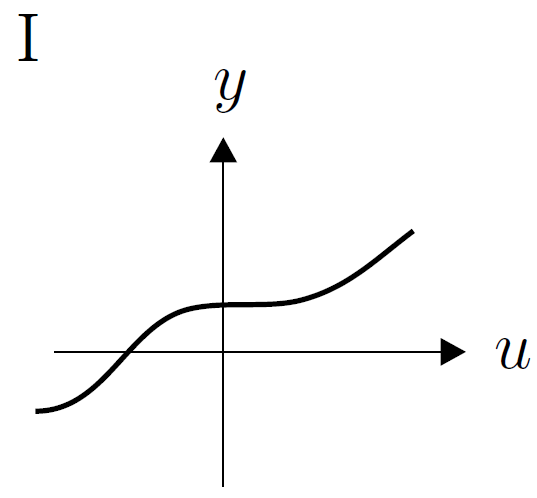
\includegraphics[width=0.85\columnwidth]{images/kennlinie.png}
    \end{center}
\end{minipage}
\hfill
\begin{minipage}[t]{0.7\columnwidth}
    \begin{center}
        \subsubsection{Pseudostatische Kennlinien}
        
        \vspace{-0.4cm}
        $$ \boxed{\text{Nicht mathematisch beschreibbar} }$$

        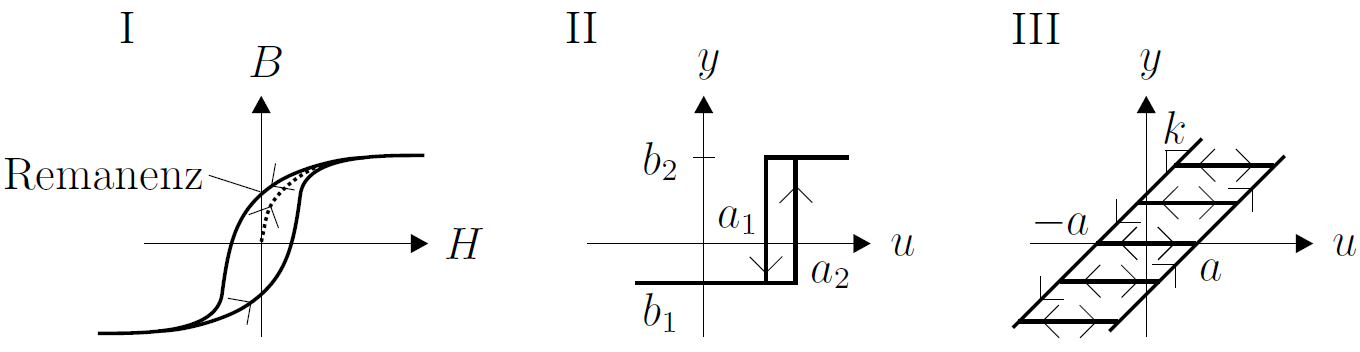
\includegraphics[width=\columnwidth]{images/pseudokennlinien.png}
    \end{center}
\end{minipage}

